%% LyX 2.3.2 created this file.  For more info, see http://www.lyx.org/.
%% Do not edit unless you really know what you are doing.
\documentclass[12pt,oneside,spanish,oldfontcommands]{memoir}
%\usepackage[authoryear]{natbib}
\usepackage[utf8]{inputenc}
\usepackage[backend=biber,style=apa]{biblatex}
\addbibresource{referencias.bib}
\DeclareLanguageMapping{spanish}{spanish-apa}
\usepackage{mathpazo}
\usepackage[T1]{fontenc}
\setcounter{secnumdepth}{3}
\setcounter{tocdepth}{3}
\setlength{\parskip}{\medskipamount}
\setlength{\parindent}{0pt}
\usepackage{babel}
\usepackage{blindtext}
\usepackage{tabu}
\usepackage{booktabs}% for better rules in the table
\usepackage{float}
\usepackage{url}
 
\DeclareUnicodeCharacter{0301}{*************************************}
 
 
\usepackage{endnotes}
\addto\shorthandsspanish{\spanishdeactivate{~<>.}}

\usepackage{array}
\usepackage{rotfloat}
\usepackage{booktabs}
\usepackage{textcomp}
%\usepackage{amssymb,amsmath}
%\usepackage[fixamsmath]{mathtools}
%  \mathtoolsset{showmanualtags,mathic,centercolon}
\usepackage{graphicx}
\usepackage{esint}
\usepackage{csquotes}
\usepackage{hyperref} % paquete para links
\usepackage[none]{hyphenat} % evitar cortes de palabras
\usepackage{longtable}

%%% agregados aaparte 

\usepackage{dsfont}
\usepackage{algorithm}
\usepackage{multirow}
%\usepackage{algorithmic}
\usepackage{algorithmicx}
\usepackage{algpseudocode}


\algdef{SE}[VARIABLES]{Variables}{EndVariables}
   {\algorithmicvariables}
   {\algorithmicend\ \algorithmicvariables}
\algnewcommand{\algorithmicvariables}{\textbf{global variables}}


\newcommand{\Tau}{\mathrm{T}}
\newcommand{\I}{\mathds{1}}
\usepackage{mathpazo}

% Example environments ---------------------------------------------------------
\RequirePackage{fancyvrb}
\RequirePackage{alltt}

\DefineVerbatimEnvironment{example}{Verbatim}{fontsize=\scriptsize}
\renewenvironment{example*}{\begin{alltt}}{\end{alltt}}

% Support for output from Sweave, and generic session style code
% These used to have fontshape=sl for Sinput/Scode/Sin, but pslatex
% won't use a condensed font in that case.

% Update (2015-05-28 by DS): remove fontsize=\small to match example environment

\DefineVerbatimEnvironment{Sinput}{Verbatim}{}
\DefineVerbatimEnvironment{Soutput}{Verbatim}{}
\DefineVerbatimEnvironment{Scode}{Verbatim}{}
\DefineVerbatimEnvironment{Sin}{Verbatim}{}
\DefineVerbatimEnvironment{Sout}{Verbatim}{}
\newenvironment{Schunk}{}{}


\makeatletter
%%%%%%%%%%%%%%%%%%%%%%%%%%%%%% LyX specific LaTeX commands.
%% Because html converters don't know tabularnewline
%% aqui comentado

%\providecommand{\tabularnewline}{\\}
%\floatstyle{ruled}
%\newfloat{algorithm}{tbp}{loa}[chapter]
%\providecommand{\algorithmname}{Algoritmo}
%\floatname{algorithm}{\protect\algorithmname}

%%%%%%%%%%%%%%%%%%%%%%%%%%%%%% Textclass specific LaTeX commands.
%\theoremstyle{plain}
%\newtheorem{thm}{\protect\theoremname}
%\theoremstyle{definition}
%\newtheorem{defn}[thm]{\protect\definitionname}

\@ifundefined{showcaptionsetup}{}{%
 \PassOptionsToPackage{caption=false}{subfig}}
\usepackage{subfig}
\makeatother


\usepackage{listings}
\providecommand{\definitionname}{Definición}
\providecommand{\theoremname}{Teorema}
\renewcommand{\lstlistingname}{Listado de código}




\makeatletter
\renewcommand{\ALG@name}{Algoritmo}
\makeatother

\begin{document}
% lo dejo como cuadro o tabla?
%\renewcommand{\listtablename}{Índice de tablas}
%\renewcommand{\tablename}{Tabla}

\sloppy % ajusta texto a los márgenes
\vspace*{-6\baselineskip}
\pagenumbering{gobble}
\hspace*{-0.0\textwidth}
\includegraphics[width=\textwidth]{images/Logo_depto_ing_informatica.png}\nonumber

\vspace{3cm}

\begin{center}
    \textbf{ RECURSO PARA EL MANEJO DE DOCUMENTOS TRIBUTARIOS ELECTRÓNICOS DEL SERVICIO DE IMPUESTOS INTERNOS DE CHILE PARA LA INTEGRACIÓN EN SISTEMAS INFORMÁTICOS BAJO EL RÉGIMEN DE LA NORMATIVA COMERCIAL Y TRIBUTARIA CHILENA}
\end{center}
\vspace{3.5cm}

\begin{center}
por
\par\end{center}

\begin{center}
JORGE OSVALDO ARIAS LEAL\vspace{3cm}
\par\end{center}

\begin{center}
Trabajo de Título presentado a la\\
Facultad de Ingeniería de la Universidad Católica de Temuco\\
Para Optar al Título de Ingeniero Civil Informático.
\par\end{center}
\begin{center}
- Temuco, MES AÑO -
\par\end{center}


\begin{center}
\vspace*{-9\baselineskip}
\hspace*{-0.1\textwidth}

\includegraphics[width=0.8\textwidth]{images/Logo_depto_ing_informatica.png}\nonumber\\
\textbf{COMISION EXAMEN DE TITULO}
\par\end{center}

Este Examen de Título ha sido realizado en la Escuela de Ingeniería Informática:
\vspace{0.4cm}

\begin{tabular}{>{\raggedright}p{0.4\columnwidth}>{\centering}p{0.7\columnwidth}}
Presidente Comisión: & .............................................................................\tabularnewline
 & \textbf{Prof. Marcos Lévano Huamaccto}\\
Magíster en Ingeniería en Informática\\
Ingeniero Informático\\
Jefe Carrera Ing. Civil Informática\tabularnewline
 & \tabularnewline
 & \tabularnewline
Profesor Guía: & .............................................................................\tabularnewline
 & \textbf{Prof. Nombre del Prof. Guía de Trabajo de Título}\\
Título Profesional \\
Título de Posgrado más Alto \tabularnewline
 & \tabularnewline
 & \tabularnewline
Profesor Informante: & .............................................................................\tabularnewline
 & \textbf{Prof. Nombre del Informante de Trabajo de Título}\\
Título Profesional \\
Título de Posgrado más Alto\tabularnewline
 & \tabularnewline
 & \tabularnewline
Jefe Carrera de Ingeniería Civil Informática: & .............................................................................\tabularnewline
 & \textbf{Sr. Marcos Lévano Huamacctoa}\\
Magíster en Ingeniería en Informática\\
Ingeniero Informático\\
Jefe Carrera Ing. Civil Informática\tabularnewline
\vspace{8mm}
\end{tabular}
Temuco, día de mes de año.\\

%R. Ortega 02950  www.inf.uct.cl/ Fono 205414-  http://www.uct.cl / Casilla 15-D / Temuco /Chile


\begin{center}
\vspace*{-9\baselineskip}
\hspace*{-0.1\textwidth}

\includegraphics[width=0.8\textwidth]{images/Logo_depto_ing_informatica.png}\nonumber\\
\textbf{INFORME  TRABAJO  DE TITULO}
\par\end{center}

\vspace{1cm}

\begin{tabular}{>{\raggedright}p{0.2\columnwidth}>{\raggedright}p{0.01\columnwidth}>{\raggedright}p{0.79\columnwidth}}
TITULO & : & ``TÍTULO DEL TRABAJO DE TÍTULO''\tabularnewline
 &  & \tabularnewline
ALUMNO & : & NOMBRE DEL ESTUDIANTE\tabularnewline
\end{tabular}

\vspace{1cm}

En mi calidad de Profesor Guía, mis apreciaciones del presente informe de Trabajo de Titulo, son las siguientes:
\begin{itemize}
    \item Apreciación 1.
    \item Apreciación 2. 
    \item Apreciación 3.
    \item Etc...
\end{itemize}


De acuerdo a estas consideraciones califico el desarrollo de este Trabajo de Título con \textbf{nota X,X  (nota en letras).}

\vspace{1cm}

\begin{flushright}
\rule{65mm}{0.2mm}\\
\end{flushright} 
\vspace*{-0.1in}  
\hspace*{3.2in} \textbf{Prof. Nombre del Prof. Guía} \\  
\hspace*{3.5in} \textbf{Profesor Guía}

\vspace{1cm}

Temuco, dia de mes de año.




\begin{center}
\vspace*{-9\baselineskip}
\hspace*{-0.1\textwidth}

\includegraphics[width=0.8\textwidth]{images/Logo_depto_ing_informatica.png}\nonumber\\
\textbf{INFORME  TRABAJO  DE TITULO}
\par\end{center}

\newcommand{\SubItem}[1]{
    {\setlength\itemindent{15pt} \item[-] #1}
}
\vspace{0.8cm}

\begin{tabular}{>{\raggedright}p{0.2\columnwidth}>{\raggedright}p{0.01\columnwidth}>{\raggedright}p{0.79\columnwidth}}
TITULO & : & ``TÍTULO DEL TRABAJO DE TÍTULO''\tabularnewline
 &  & \tabularnewline
ALUMNO & : & NOMBRE DEL ESTUDIANTE\tabularnewline
\end{tabular}

\vspace{1cm}

En mi calidad de Profesor Informante, mis apreciaciones del presente informe de Trabajo de Titulo, son las siguientes:
\begin{itemize}
    \item Apreciación 1.
    \item Apreciación 2. 
    \item Apreciación 3.
    \item Etc...
\end{itemize}

De acuerdo a estas consideraciones califico el desarrollo de este Trabajo de Título con \textbf{nota X,X  (nota en letras).}

\vspace{1cm}

\begin{flushright}
\rule{65mm}{0.2mm}\\
\end{flushright} 
\vspace*{-0.1in}  
\hspace*{2.8in} \textbf{Prof. Nombre del Profesor Informante} \\ \hspace*{3.2in} \textbf{Profesor Informante}

\vspace{1cm}

Temuco, día de mes de año.


\thispagestyle{empty}
\begin{center}
\textbf{AGRADECIMIENTOS}
\par\end{center}

A todos aquellos que, a través de la educación, han logrado cambiar realidades como la mía y, sabiendo su impacto, continuarán transformando el mundo.

\pagebreak{}

\pagenumbering{roman}

\tableofcontents{}

\pagebreak{}

\listoffigures

\pagebreak{}

\listoftables

\pagebreak{}

%\renewcommand{\listalgorithmname}{Índice de algoritmos}
%\listofalgorithms
%\addcontentsline{toc}{chapter}{Índice de algoritmos}
%\pagebreak{}

\thispagestyle{plain} % don't show page number
\clearpage 

\begin{abstract}
\addcontentsline{toc}{chapter}{Resumen}
Resumen en español.


{\bf Palabras Clave:} 
Palabras claves en español, separadas por coma.
\end{abstract}


\pagebreak{}

\thispagestyle{plain} % don't show page number
\clearpage 
\renewcommand{\abstractname}{Abstract}
\begin{abstract}
\addcontentsline{toc}{chapter}{Abstract}


{\bf Keywords:} 
DTE, SII, management, integration, resource.
\end{abstract}
\addto{\captionsspanish}{\renewcommand{\abstractname}{Executive Summary}}

\pagebreak{}

\pagenumbering{arabic}
\setcounter{page}{1}

\chapter{Introducción}

\section{Problema}

%% cite{Infórmate} como \texcite o como \parencite
La Ley Nº 20.727 de 2014 establece el uso obligatorio de la factura electrónica, junto a otros documentos tributarios electrónicos como liquidación factura, notas de débito y crédito y factura de compra. Para las grandes empresas el plazo de incorporación venció en 2014, para las Medianas y Pequeñas Empresas el año 2016 y 2017 y para las Microempresas hasta el año 2017 y 2018.

Esta implementación posiciona a Chile como uno de los países con mayor y más temprana adopción a la digitalización en Latinoamérica, lo que impulsa a las empresas a mejorar los procesos de gestión de la información, tanto internamente como en el cumplimiento de las regulaciones fiscales del país. Sin embargo, también conllevan a establecer una barrera de entrada para nuevas empresas, las que deben ser digitales desde el día cero para comenzar a operar. Y es un desafío constante a mantener un sistema que permita dar cumplimiento con lo que dispone el Servicio de Impuestos Internos de Chile en cuanto a dichas regulaciones de manejo y presentación de documentos tributarios.

De acuerdo con las estadísticas publicadas por el Servicio de Impuestos Internos (SII) en su portal oficial sobre Factura Electrónica \textcite{estadisticasFacturaElectronica} \footnote{Ver \url{https://www.sii.cl/servicios_online/1039-estadistic-1182.html}}, se destacan los siguientes datos relevantes:
\begin{enumerate}
	\item Durante el año 2023, se inscribieron en Factura Electrónica 137.714 empresas.
	\item De los contribuyentes inscritos durante el año 2023, el 94,56\% lo hizo a través del Sistema de Facturación Gratuito del SII.
	\item Durante el año 2023, se emitieron más de 695 millones de Documentos Tributarios Electrónicos.
	\item El 9\% de las empresas habilitadas utilizan software de mercado o propio, mientras que el otro 91\% utiliza el Sistema de Facturación gratuito otorgado por el SII.
	\item El 79\% de las empresas habilitadas corresponde a grandes empresas, mientras que el 21\% corresponde a Medianas y Pequeñas Empresas, y Microempresas. Esto sugiere que la mayoría de las grandes empresas aún no implementan una solución de software propio que se integre directamente con sus sistemas de gestión internos.
	\item En el año 2024, únicamente 11.076 empresas implementaron un software de mercado o propio, mientras que 85.583 fueron habilitados como emisores de factura electrónica a través del Sistema de Facturación Gratuito del SII.
	\item El 58\% de los DTE emitidos corresponden únicamente al de tipo Factura Electrónica.
\end{enumerate}

La obligación de cumplir con la emisión de DTE, junto con la evidencia de la baja adopción de integraciones con software de mercado o propio —un hecho que se contradice con las necesidades de un comercio interconectado y beneficiado por la digitalización—, hace necesario desarrollar una solución que permita a las empresas implementar y gestionar eficientemente sus DTE, además de integrarlas con la amplia variedad de soluciones digitales disponibles para la gestión de procesos y comercio.

Los constantes avances tecnológicos continúan siendo una parte crucial en la optimización de los costos operativos para las empresas. Estas han ido evolucionando, haciendo cada vez más necesaria una mayor integración entre sistemas de la misma o diferentes entidades. Actualmente, la incorporación de análisis de datos avanzados y la inteligencia artificial se han ido adoptando en búsqueda de optimizar la toma de decisiones, aumentar la precisión y eficiencia, y avanzar hacia la automatización y autonomía en la gestión y operación de las empresas.

\section{Antecedentes}

En el mercado de software empresarial actual, existe una gran cantidad de programas que permiten mejorar la gestión empresarial tanto en la parte administrativa como en el proceso. Existen sistemas gratuitos como Odoo (ex OpenERP) que permiten gestionar la información de una empresa, están calificados como sistemas  de clase mundial, pero que por lo mismo no están concretamente diseñados para adaptarse a la normativa comercial y tributaria chilena y no adoptan de manera nativa la actual integración de documentación tributaria electrónica que exige el Servicio de Impuestos Internos.

También existen sistemas de pago ofrecidos por empresas como SAP, Oracle, QAD, Softland, Microsoft, entre otros; pero que no logran llegar a las MiPyME (Pequeñas Medianas y Microempresas) debido a su alto costo de mercado, plataforma y mantención. Y para algunas de las grandes empresas, estas no permiten realizar una integración adecuada a sistemas informáticos propios o no les permite adoptar rápidamente los cambios necesarios cuando el Servicio de Impuestos Internos aplica nuevos requisitos a la regulación.

Para facilitar la adopción a las PyME y Microempresas el Servicio de Impuestos Internos ha puesto a disposición de los contribuyentes un sistema de facturación gratuito de funcionalidad básica, que les permite operar con facturas electrónicas y cumplir con la normativa que el SII ha establecido para los contribuyentes autorizados a emitir documentos tributarios electrónicos, pero que no permite integrar funcionalidades acordes a las necesidades de cada empresa y compatibles con sus propios sistemas.

Como solución para la implementación en el desarrollo de software propio, existió una librería DTE para Java creada por NicLabs en el año 2011. Actualmente se encuentra deprecada desde Enero del 2017 y ya no recibe actualizaciones para la solución de incidencias, pero aparentemente funcional aún corrigiendo algunas definiciones deprecadas u otras incidencias, pero sin ninguna garantía.

Empresas como Acepta.com S.A. y SOVOS ofrecen soluciones de facturación electrónica de pago en forma de Web Service, enfocada principalmente en el segmento de mercado de las medianas y grandes empresas. Aunque, según la evidencia de adopción de software de mercado, el Software de Facturación gratuito ofrecido por el SII continúa siendo la solución predominante para complir con la obligación, a pesar de sus limitaciones.

\section{Objetivos}

\subsection{Objetivo general}

\begin{itemize} 
    \item Desarrollar un recurso para la implementación de Documentación Tributaria Electrónica que cumpla con los estándares exigidos por el Servicio de Impuestos Internos y permita a las empresas dar cumplimiento a su obligación de adopción según las normas y requisitos establecidos, además de gestionar y resguardar eficazmente dicha documentación tributaria e información asociada, escalable al uso e implementación tanto en grandes empresas como en PyME y Microempresas.
\end{itemize}

\subsection{Objetivos específicos}

\begin{itemize}
	\item Analizar los sistemas y recursos informáticos actuales que emplean las empresas para gestionar documentos fiscales y determinar cómo los implementan.
	\item Estudiar las necesidades y estado actual de las empresas en cuanto a la normativa vigente para cumplir con la documentación electrónica.
	\item Desarrollar una librería y/o servicio informático que permita realizar las operaciones que indica el Servicio de Impuestos Internos para la implementación de Documentación Tributaria Electrónica.
	\item Implementar estándares técnicos que garanticen calidad, seguridad, escalabilidad y resiliencia.
	\item Validar que la solución desarrollada pueda ser integrada técnicamente en los sistemas de las empresas.
\end{itemize}
\chapter{Marco teórico}
\section{Contenido del marco teórico}
El marco teórico debe explicar, clara y resumidamente, el conocimiento necesario para poder entender el trabajo de título realizado. Puede tocar aspectos matemáticos, informáticos o, por lo general, ambos. Las ecuaciones utilizadas deben ser numeradas y etiquetadas para poder usar referencias cruzadas.

Por ejemplo: 
La Teoría de los Efectos Olvidados fue propuesta por \textcite{kaufmann1988modelos} para identificar efectos indirectos a partir de procesos causa-efecto.

Los efectos olvidados de segundo orden se calculan mediante
\begin{equation}
    CE^{n+1}= CE^{\sum_{i=1}^{n+1}{i}} - CE^{\sum_{i=1}^n{i}}
\end{equation}

donde:
\begin{equation}
    CE^{\sum_{i=1}^{n+1}{i}} = CC \circ CE^{\sum_{i=1}^n{i}} \circ EE
    \label{eq: maxmin_triple}
\end{equation}

y $\circ$ es un operador no lineal y asociativo conocido como convolución maxmin. En términos generales para una matriz cuadrada y reflexiva:
\begin{equation}
    A = [ \mu_{c, \hat{c}}]_{ C \times C} 
\end{equation}

donde la convolución maxmin utilizada en \ref{eq: maxmin_triple} es definida como:

\begin{equation}
    \mu_{c,\hat{c}}^{1+2} = max_{c, \hat{c} = 1,..., C}\{ min_{k = 1,...,C}\{\mu_{c,k}, \mu_{k,\hat{c}} \} \}
    \label{eq: maxmin}
\end{equation}

y los efectos de segundo orden se obtienen de:
\begin{equation}
    \mu_{c,\hat{c}}^{2} = \mu_{c,\hat{c}}^{1+2} - \mu_{c, \hat{c}}
\end{equation}

\section{Figuras\label{Sec: Figuras}}
Las figuras deben ser generadas en PDF, incluidas en el documento y referenciadas usando referencias cruzadas. Por ejemplo:

La Figura \ref{figure: 1d_triangle} muestra un ejemplo simple de efectos olvidados o las relaciones indirectas entre dos nodos de una red. Dado tres nodos $A$, $B$, $C$, de un grafo, y el peso de cada arista $\mu_{a,b}$, $\mu_{a,c}$ y $\mu_{b,c}$ $\in [0\,,\,1]$ , si $min(\mu_{a,b}, \mu_{b,c}) - \mu_{a,c} > 0.5$ es posible decir que la incidencia indirecta $A \rightarrow C$ por medio de $B$ es mas fuerte que la incidencia directa $A \rightarrow C$.
\begin{figure}[H]
  \centering
  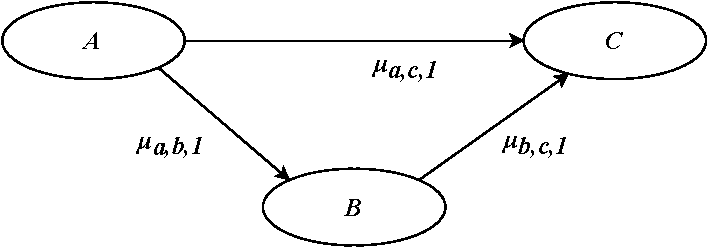
\includegraphics[width=\textwidth]{files/1d.pdf}
  \caption{Ejemplo de relaciones directas e indirectas.}
  \label{figure: 1d_triangle}
\end{figure}

\section{Refencia a secciones anteriores}
Igualmente, cualquier referencia a secciones anteriores debe ser realizada usando referencias cruzadas. Por ejemplo:

Dado que primero necesitaremos definir algunos conceptos, el algoritmo que se utilizará para el cálculo de los efectos indirectos se presentará en la Sección \ref{Sec: Figuras}. 

\section{Cuadros}

Los cuadros deben ser diseñadas de tal manera que se usen únicamente líneas horizontales, dejando las verticales para excepciones muy limitadas. Deben ser referenciadas usando referencias cruzadas. Por ejemplo:

Para el experto $i$, $\mu_{c,\hat{e},i}$ es el grado de verdad entre $[0\,,\,1]$ del enunciado ``$c$ tiene una incidencia sobre $e$'' (equivalente para las otros dos matrices). Las matrices $CC_i$ y $EE_i$ son reflexivas, es decir, son cuadradas y de diagonal igual a 1, pero no necesariamente simétricas. Se debe definir un punto $\varepsilon$ que establece el grado de verdad mínimo de incertidumbre de la afirmación ``$c$ tiene una incidencia sobre $e$''. En el Cuadro \ref{tab:Tabla-de-Verdad} se puede apreciar la tabla endecadaria habitualmente usada en entrevistas de expertos para identificar este grado de verdad \parencite{kaufmann1993tecnicas}, en donde $\varepsilon=0,5$. No obstante, el paquete puede trabajar con escalas continuas en el intervalo $[0\,,\,1]$, permitiendo un granularidad más fina en la evaluación de los grados de verdad de las relaciones y valores de $\varepsilon$ particulares para el caso estudiado.. 

\begin{table}
\centering
\begin{tabular}{|l|l|}
\hline
\textbf{Grados de Verdad} & \textbf{Evaluación}     \\ \hline
0                         & Falso                   \\ \hline
0,1                       & Prácticamente falso     \\ \hline
0,2                       & Casi falso              \\ \hline
0,3                       & Bastante falso          \\ \hline
0,4                       & Más falso que verdadero \\ \hline
0,5                       & Ni verdadero ni falso   \\ \hline
0,6                       & Más verdadero que falso \\ \hline
0,7                       & Casi verdadero          \\ \hline
0,8                       & Bastante verdadero      \\ \hline
0,9                       & Prácticamente verdadero \\ \hline
1                         & Verdadero               \\ \hline
\end{tabular}
\caption{Tabla endecadaria de grados de verdad.}
\label{tab:Tabla-de-Verdad}
\end{table}

\section{Algoritmos}
Los algoritmos deben ser presentados en un pseudo-código muy resumido, prefiriendo la notación matemática en su lugar. Deben ser creados usando las clases \texttt{algorithm} y \texttt{algorithmic}, así como ser referenciados usando referencias cruzadas.

La matriz conjugada de orden $n$, $CE^{\sum_{i=1}^{n}{i}}$, contiene todos los efectos directos y olvidados que se han encontrado hasta ese momento. Para encontrar $CE^{n+1}$, debe sustraerse de la matriz conjugada de orden $n+1$ la matriz conjugada de orden $n$. Se actualiza, tomando como referencia $\varepsilon$, la lista de efectos de orden $n+1$ según el Algoritmo \ref{FE.recursive}. $CE^{n+1}$ es una matriz de ceros únicamente cuando ya no existen efectos olvidados de grado $n+1$ o superior, por lo que el algoritmo se detiene y retorna los efectos olvidados identificados en la lista $edges$.

\begin{algorithm}
\begin{algorithmic}[1]
\caption{\textsc{FE.recursive}}
\label{FE.recursive}
\Variables
 \State $n$
 \State $edges$
\EndVariables
\Procedure{FE.recursive}{$CC_{i}, CE^{\sum_{i=1}^n{i}}, EE_{i}, \varepsilon \in [0,1], maxOrder \geq 2, CE^{n}$}
\State $n \Leftarrow n + 1$
%\State $edges \Leftarrow$ elements of $CE^n> \varepsilon$
\If{ $\left| \textbf{ elements of } CE^n > \varepsilon \right| = 0 \textbf{ or } n \geq maxOrder + 1$}
    \State \textbf{return} $edges$ 
\EndIf
    %\State $CE^{\sum_{i=1}^{n+1}{i}} \Leftarrow$ \Call{maxmin}{\Call{maxmin}{$CC_{i},CE^{\sum_{i=1}^n{i}}$}$,EE_{i}$}
    \State $CE^{\sum_{i=1}^{n+1}{i}} \Leftarrow$ \textsc{maxmin}(\textsc{maxmin}($CC_{i},CE^{\sum_{i=1}^n{i}}$)$,EE_{i}$)
    \State $CE^{n+1} \Leftarrow CE^{\sum_{i=1}^{n+1}{i}} - CE^{\sum_{i=1}^n{i}}$
    \State \Call{FE.recursive}{$CC_{i}, CE^{\sum_{i=1}^{n+1}{i}}, EE_{i}, \varepsilon, maxOrder,CE^{n+1}$}
    %\State \textbf{Update} $edges$  \textbf{with elements of}   $CE^{n+1}> \varepsilon$
    %\State \textbf{Update} $FE.list$ \textbf{with} $\Call{Seek.Paths}{edges, CC_{i}, CE^{\sum_{i=1}^{n}{i}}, EE_{i}, CE^{n+1}}$
    \State $n \Leftarrow n - 1$
    
    \State \textbf{Update} $edges \textbf{ with elements of } CE^{n+1} \geq \varepsilon$
    
    \State \textbf{Update} $edges$ \textbf{with} $\Call{Seek.Paths}{edges, CC_{i}, CE^{\sum_{i=1}^{n+1}{i}}, EE_{i}, CE^{n+1}}$

\State \textbf{return} $edges$
\EndProcedure
\end{algorithmic}
\end{algorithm}


\chapter{Resultados}

\chapter{Discusión y Análisis de Resultados}
Los resultados deben ser análizados en función del problema estudiado. Su discusión, en la medida de lo posible, debe ir acompañada de referencias bibliográficas relevantes, aunque esto debe ser determinado caso a caso. Por ejemplo:

Los resultados son concluyentes, los efectos directos sugieren que la subvención al transporte (\texttt{I14}) no tiene ningún efecto sobre reducir la contaminación del aire en áreas residenciales. Por otro lado, la educación (\texttt{I11}), I+D investigación y desarrollo (\texttt{I13}) y la mitigación (\texttt{I16}), si tienen un efecto directo sobre reducir la contaminación del aire. Los efectos olvidados sugieren que si la gente mejora el aislamiento térmico de sus casas (\texttt{B1}), puede contribuir a una reducción mayor de la contaminación del aire. Los sistemas de evaluación de impacto ambiental (\texttt{I15}), educación (\texttt{I11}) y I+D investigación y desarrollo (\texttt{I13}) también pueden desempeñar un papel importante para fomentar el cambio de comportamiento ya que aparecen como intermediarios entre las relaciones de origen asociadas a los incentivos, mejora y producción (\texttt{I8}), subvención para leña (\texttt{I9}) y el destino asociado al comportamiento \texttt{B1}

\chapter{Conclusiones}

\section{Trabajo Futuro}

\subsection{Extensión de Implementaciones en otros Sistemas y Tecnologías}

\subsection{Implementación sobre Arquitectura basada en Microservicios propuesta}

\subsection{Integración con Sistemas de Análisis de datos}

\subsection{Integración con Modelos de Inteligencia Artificial}


\printbibliography
%\bibliographystyle{plainnat}
%\bibliography{referencias.bib}


%
\chapter{Anexos}
\begin{table}[]
\centering
\caption{Primeros 20 elementos con orden creciente}
\label{tab: directCHICO}
\begin{tabular}{llllll}
    & From & To  & Mean  & UCI    & p.value  \\
207 & I14  & I12 & 0.12  & 0.21   & 0.00416  \\
199 & I14  & I4  & 0.125 & 0.205  & 0.00253  \\
58  & I4   & I14 & 0.14  & 0.24   & 0.00485  \\
43  & I3   & I14 & 0.145 & 0.26   & 0.00621  \\
148 & I10  & I14 & 0.145 & 0.255  & 0.00429  \\
290 & I14  & B2  & 0.145 & 0.24   & 0.00312  \\
289 & I14  & B1  & 0.155 & 0.255  & 0.00258  \\
205 & I14  & I10 & 0.16  & 0.28   & 0.00273  \\
198 & I14  & I3  & 0.17  & 0.28   & 0.00168  \\
178 & I12  & I14 & 0.18  & 0.285  & 0.00102  \\
196 & I14  & I1  & 0.18  & 0.265  & 0.000649 \\
133 & I9   & I14 & 0.185 & 0.29   & 0.00244  \\
204 & I14  & I9  & 0.195 & 0.345  & 0.00521  \\
291 & I14  & B3  & 0.21  & 0.3714 & 0.0119   \\
88  & I6   & I14 & 0.23  & 0.355  & 0.00233  \\
200 & I14  & I5  & 0.23  & 0.38   & 0.00389  \\
203 & I14  & I8  & 0.235 & 0.355  & 0.00166  \\
269 & I9   & B1  & 0.235 & 0.4    & 0.00725  \\
201 & I14  & I6  & 0.245 & 0.4    & 0.00618  \\
181 & I13  & I1  & 0.255 & 0.355  & 0.00175 
\end{tabular}
\end{table}

% Please add the following required packages to your document preamble:
% \usepackage{graphicx}
\begin{table}[]
\centering
\caption{Primeros 20 elementos con orden decreciente}
\label{tab: directGRANDE}
\begin{tabular}{llllll}
    & From & To  & Mean  & UCI   & p.value \\
280 & I11  & B4  & 0.975 & 0.985 & 0.984   \\
273 & I10  & B1  & 0.915 & 0.965 & 0.986   \\
259 & I6   & B3  & 0.9   & 0.945 & 0.994   \\
288 & I13  & B4  & 0.9   & 0.95  & 0.985   \\
285 & I13  & B1  & 0.885 & 0.945 & 0.998   \\
286 & I13  & B2  & 0.885 & 0.94  & 0.998   \\
287 & I13  & B3  & 0.885 & 0.945 & 0.993   \\
279 & I11  & B3  & 0.875 & 0.93  & 0.998   \\
267 & I8   & B3  & 0.835 & 0.905 & 0.999   \\
308 & B3   & B2  & 0.835 & 0.875 & 0.992   \\
191 & I13  & I11 & 0.83  & 0.92  & 0.99    \\
248 & I3   & B2  & 0.825 & 0.88  & 0.997   \\
21  & I2   & I7  & 0.82  & 0.885 & 0.999   \\
312 & B4   & B3  & 0.82  & 0.9   & 0.999   \\
6   & I1   & I7  & 0.815 & 0.87  & 1       \\
251 & I4   & B2  & 0.815 & 0.88  & 0.998   \\
263 & I7   & B3  & 0.815 & 0.88  & 0.998   \\
277 & I11  & B1  & 0.81  & 0.915 & 0.974   \\
278 & I11  & B2  & 0.81  & 0.91  & 0.955   \\
311 & B4   & B2  & 0.805 & 0.885 & 0.998  
\end{tabular}
\end{table}

\end{document}
